Quanten Computing ist eine relativ junge Disziplin der Physik und Informatik. Obwohl die Entwicklung der beiden Bereiche unabhängig voneinander zu Beginn des 20. Jahrhunderts begann, wurden schon in den 1980er Jahren die ersten Versuche unternommen und theoretische Überlegungen angestellt, um Methoden der Informatik mithilfe von Quantenobjekten umzusetzen. Obwohl der \ac{qc} erst seit kurzer Zeit existiert, hat er bereits bedeutende Fortschritte gemacht und besitzt ein enormes Potenzial für Entwicklungen zum Beispiel in den Bereichen Kryptographie, Optimierungsprobleme, Simulation chemischer Prozesse und maschinelles Lernen.

\subsection{Ein theoretischer \ac{qc}}
Ein der Informatik zugrunde liegendes Prinzip ist, dass \cite[S122]{steane_quantum_1998} Informationen auf unterschiedlichen Weisen dargestellt (codiert) werden können. So kann die Zahl \textit{fünf} zum Beispiel binär ($0101$) oder als Unicode Zeichen (\textit{U+0035}) dargestellt werden. Der Inhalt der Information ist in beiden Fällen jedoch der Gleiche.\\
Dieses Prinzip ist für die Informatik sehr wichtig. Es ermöglicht Maschinen komplexe Informationen zu speichern, mithilfe einfacher Operationen zu manipulieren und wieder in ein komplexes Format zu überführen, ohne dabei an Informationsgehalt zu verlieren oder Informationen unkenntlich zu machen. In einem Computer werden diese Informationen in Form von \textit{bits} darstellt die zwei Zustände, repräsentiert durch \textit{0} und \textit{1}, annehmen können. In einem klassischen, digitalen Computer sind diese beispielsweise durch das fließen von Strom abgebildet. Ein \ac{qc} repräsentiert Informationen in den Eigenschaften von Quanten-Objekten, beispielsweise dem Spin von Elektronen.\\
%% Universaler \ac{qc} ???
Um die Funktion eines \ac{qc} zu erläutern muss erst ein kurzer Blick auf einige quantenphysikalische Phänomene geworfen werden.

\subsubsection{Superpositionen}
Eine Superposition ist das Fundamentale quantenphysische Phänomen das einem \ac{qc} zugrunde Liegt.
Es wird meistens mithilfe des Gedankenexperiments von \cite[\$5]{schrodinger_gegenwartige_1935} \textit{Schrödingers Katze} veranschaulicht: In einer Box befindet sich eine Katze und ein Gefäß mit Gift das zerstört wird und die Katze tötet, wenn ein radioaktiver Zerfall gemessen wird. Außerhalb der Box lässt sich nicht feststellen, ob der Mechanismus der das Gift freisetzt aktiviert wurde. Sie befindet sich, Quantenmechanisch gesehen, in einem Zustand in dem sie sowohl tot als auch lebendig ist. In dem Moment, in dem die Box geöffnet wird, kann festgestellt werden welcher der beiden Zustände eingetroffen ist.\\
Auf ein Quantenteilchen übertragen heißt das: Es kann sich in einem undefinierten Zustand befinden, der \textbf{Superposition} aus allen möglichen Zuständen. Erst wenn \textit{nachgeschaut}, also der Zustand gemessen wird, kollabiert die Superposition in einen der möglichen Zustände. Eine Superposition kann durch die Wahrscheinlichkeit, mit der jeder der Zustände eintreten kann, beschrieben werden. Ein Elektron mit den Zuständen Spin up ($75\%$) und Spin down ($25\%$) kollabiert also, wenn der Spin gemessen wird zu $3/4$ der Fälle als Spin up und zu $1/4$ als Spin down.
Mathematisch kann eine Superposition $\psi$ als Linearkombination ihrer Zustände betrachtet werden. 
\begin{equation}
    \ket{\psi } = \alpha \ket{1} + \beta \ket{0} \\
\end{equation}
Diese Linearkombination kann auch grafisch, als Vektor auf einer Kugel dargestellt werden (siehe Graphik \ref{fig:spin}). Es ist zu beachten, dass der Vektor \textit{z} nicht den Spin, sondern die Linearkombination darstellt.

\begin{figure}[!hbt]
    \centering
    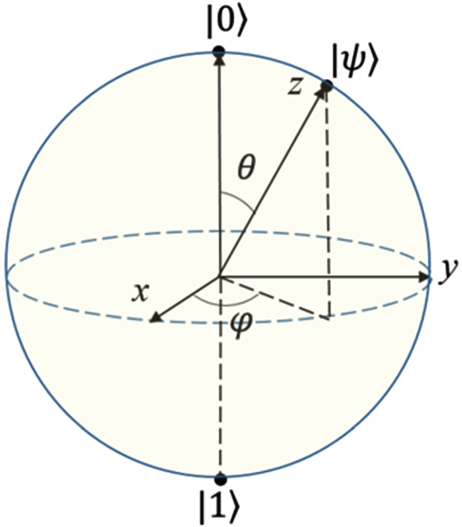
\includegraphics{./images/spin-superpostition.jpg}
    \caption{Spin eines Elektrons in Superposition \cite{noauthor_cpb_27_9_090308_f8jpg_nodate}}
    \label{fig:spin}
\end{figure}

\subsubsection{Quantenverschränkung}


\subsection{Implementierung eines \ac{qc}s}


% Notes: 
% Herausforderung, warum ein QC allein noch nicht den Prozess beschleunigt. Die Herausforderung aus der Superposition aller möglichen Lösungen, die eine richtige zu erhalten.

% ChatGPT
Ein Quantenregister ist ein grundlegender Bestandteil eines Quantencomputers und repräsentiert den Speicher für Quanteninformationen. Es ist vergleichbar mit einem klassischen Register in einem herkömmlichen Computer, jedoch basiert es auf den Prinzipien der Quantenmechanik.

Ein Quantenregister besteht aus einer Anordnung von Qubits, den grundlegenden Informationseinheiten in einem Quantencomputer. Ein Qubit kann sich im Gegensatz zu einem klassischen Bit nicht nur in den Zuständen 0 oder 1 befinden, sondern es kann auch eine Überlagerung dieser Zustände bilden. Das bedeutet, dass ein Qubit gleichzeitig in einer Linearkombination von 0 und 1 existieren kann, was als Superposition bezeichnet wird. Darüber hinaus können Qubits miteinander verschränkt sein, was bedeutet, dass der Zustand eines Qubits von dem Zustand anderer Qubits abhängen kann.

Das Quantenregister dient als Container, um eine bestimmte Anzahl von Qubits zu speichern und sie miteinander zu manipulieren. Die Anzahl der Qubits in einem Quantenregister bestimmt die Größe und Komplexität der berechnungen, die ein Quantencomputer durchführen kann. Je größer das Quantenregister ist, desto mehr Qubits stehen zur Verfügung, um komplexe Berechnungen durchzuführen.

Durch die Anwendung von Quantengattern, wie beispielsweise Hadamard-Gattern, CNOT-Gattern und Phasengattern, können Operationen auf den Qubits im Quantenregister ausgeführt werden. Diese Gatter ermöglichen es, Qubits zu verschränken, Superpositionen zu erzeugen und gezielte Manipulationen der Quanteninformationen durchzuführen.

Das Quantenregister spielt eine zentrale Rolle in Quantenalgorithmen, da es die Plattform bietet, auf der die Quantenberechnungen durchgeführt werden. Die Größe und Qualität des Quantenregisters sind entscheidend für die Leistungsfähigkeit eines Quantencomputers. Daher ist die Entwicklung und Skalierung von Quantenregistern ein aktiver Bereich der Forschung, um die Möglichkeiten der Quantencomputertechnologie weiter zu verbessern.

%Quellen:
%[1] Nielsen, M. A., & Chuang, I. L. (2010). Quantum Computation and Quantum Information. Cambridge University %Press.
%[2] Mermin, N. D. (2007). Quantum Computer Science: An Introduction. Cambridge University Press.
%[3] Kaye, P., Laflamme, R., & Mosca, M. (2007). An Introduction to Quantum Computing. Oxford University Press.
